\documentclass[usenames,dvipsnames]{beamer}
\usetheme{Warsaw}
\usepackage{lmodern}
\usepackage[squaren,Gray]{SIunits}
\usepackage{amsmath}
\usepackage[utf8]{inputenc}

\newcommand{\norm}[1]{\left\lVert#1\right\rVert}


%Information to be included in the title page:
\title{Online Estimation of Inertial Parameters Using a Recursive Total Least-Squares Approach}
\author{François Le Rall}
\institute{Nomagic – Robotic Seminar}
\date{2019}



\begin{document}

\frame{\titlepage}

\begin{frame}
  \frametitle{References}

\begin{itemize}
  \item [2007] On-line rigid object recognition and pose estimation based on inertial parameters (D. Kubus, T. Kroger)
  \item [2008] On-Line Estimation of Inertial Parameters Using a Recursive Total Least-Squares Approach (D. Kubus, T. Kroger)
  \item [2014] Combining visual and inertial features for efficient grasping and bin-picking (D. Kubus, I. Weidauer)
  \item [2018] Real-Time Identification of Robot Payload using a Multirate Quaternion-based Kalman Filter and Recursive Total Least-Squares (S. Farsoni, C. Talignani Landi)

\end{itemize}
\end{frame}

\begin{frame}
 \frametitle{Definition of the problem}



 \begin{minipage}{.5\textwidth}
  \begin{itemize}
   \item F/T sensor Gamma measuring:
         \begin{itemize}
          \item force ${}^S f$,
          \item torque ${}^S \tau$,
          \item in the sensor frame $S$.
         \end{itemize}
   \item Payload grasped by the suction tool:
         \begin{itemize}
          \item mass $m$,
          \item center of mass ${}^S c$,
          \item moment of inertia ${}^S I$,
          \item linear acceleration ${}^S a$,
          \item angular acceleration ${}^S \alpha$,
          \item angular velocity ${}^S \omega$,
          \item gravity ${}^S g$.
         \end{itemize}
  \end{itemize}
 \end{minipage}%
 \begin{minipage}{0.5\textwidth}
  \centering
  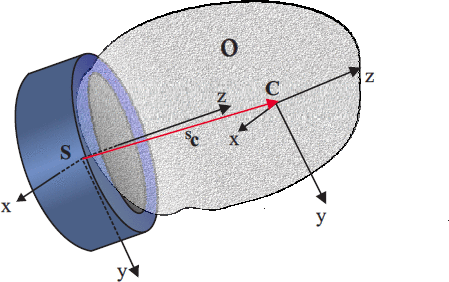
\includegraphics[scale=0.4]{images/scheme.png}
 \end{minipage}

\end{frame}

\begin{frame}
 \frametitle{Newton-Euler Approach}

 The motion of the body due to external forces is described by the two equations:

 \begin{align}
  {}^S f    & = m {}^S a - m {}^S g + {}^S \alpha \times m {}^S c + {}^S \omega \times ({}^S \omega \times m {}^S c)           \\
  {}^S \tau & = {}^S I {}^S \alpha + {}^S \omega \times ({}^S I {}^S \omega) + m {}^S c \times {}^S a - m {}^S c \times {}^S g
 \end{align}

 also in matrix form:

 \begin{equation}
  \begin{pmatrix}
   {}^S f    \\
   {}^S \tau
  \end{pmatrix}
  = {}^S A({}^S a, {}^S \alpha, {}^S \omega, {}^S g) {}^S \varphi
 \end{equation}

 with ${}^S \varphi = (m, m {}^S c_x, m {}^S c_y, m {}^S c_z, {}^S I_{xx}, {}^S I_{xy}, {}^S I_{xz}, {}^S I_{yy}, {}^S I_{yz}, {}^S I_{zz}) {}^T$
\end{frame}

\begin{frame}
 \frametitle{Estimation of the sensor offsets}
 Strain gage force/torque sensors typically show offsets that would deteriorate the estimation:
 \begin{itemize}
  \item \textcolor{red}{Zeroing the sensor value at a known sensor orientation},
  \item \textcolor{ForestGreen}{Directly estimating the sensor offsets}.
 \end{itemize}

The number of parameters to estimate increase from 10 to 16:
\begin{gather}
  {}^S \varphi_{ext} = [f_{O_x}, f_{O_y}, f_{O_z}, {}^S \varphi] {}^T \\
  {}^S A_{ext} = [\mathbb{I}_{6 \times 6} {}^S A]
\end{gather}

 {\footnotesize (drift effects can be neglected since the estimation duration is less than $3 \second$)}
\end{frame}

\begin{frame}
 \frametitle{Optimisation problem}

During the motion of the payload, $M$ ${}^S A_{ext}$ matrices are compiled at subsequent instants of time:
\begin{gather}
  {}^S A_{\Xi} = [{}^S A_1^T {}^S A_2^T \ldots {}^S A_M^T] {}^T \\
  \begin{pmatrix}
   {}^S f    \\
   {}^S \tau
  \end{pmatrix}_{\Xi}
  = \Bigg[\begin{pmatrix}
   {}^S f    \\
   {}^S \tau
  \end{pmatrix}_1^T
  \begin{pmatrix}
   {}^S f    \\
   {}^S \tau
  \end{pmatrix}_2^T
  \ldots \begin{pmatrix}
   {}^S f    \\
   {}^S \tau
  \end{pmatrix}_M^T \Bigg] {}^T
\end{gather}

The optimization problem is the following:

\begin{align*}
  \underset{{}^S \varphi}{\textrm{minimize}} \quad &
    \norm{ \begin{pmatrix}
     {}^S f    \\
     {}^S \tau
   \end{pmatrix}_{\Xi}
    - {}^S A_{\Xi} {}^S \varphi } \\
  \textrm{subject \ to} \quad & m \geq 0\\
                              & c_z \geq 0
\end{align*}

\end{frame}


\begin{frame}
 \frametitle{Recursive Total Least-Squares (RTLS) Method}
RTLS
\end{frame}

\begin{frame}
 \frametitle{}
End frame
\end{frame}

\end{document}
